\documentclass{standalone}
\usepackage{tikz}
\usepackage{calc}
\begin{document}
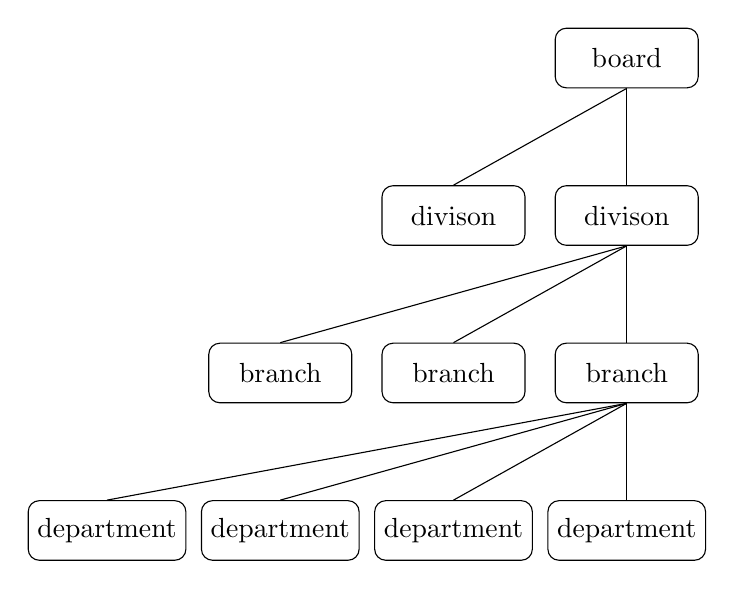
\begin{tikzpicture}
    \tikzset{
        every node/.style={
            draw,
            rounded corners,
            minimum width=12ex,
            minimum height=5ex
        }
        }
    \foreach [count=\y] \myname in {board,divison,branch,department}
    {
    \foreach \x in {1,...,\y}
        {
        \node (X\x-Y\y) at (-2.2*\x,-2*\y) {\myname};
        }
    }
    \foreach [count=\yy] \y in {2,3,4}
    {
    \foreach \x in {1,...,\y}
        {
        \draw(X1-Y\yy.south) -- (X\x-Y\y.north);
        }
    }

\end{tikzpicture}
\end{document}